Om het gebruik van de applicatie onder onze doelgroep te bevorderen is het belangrijk om de applicatie aan te laten sluiten bij de verwachtingen en eisen van onze doelgroep. Om deze reden is het uiterst belangrijk dat er in een vroeg stadium gecontroleerd wordt of de functionaliteit die gebouwd wordt, aansluit op de wensen van de gebruikers. Om deze reden zal er vlak na onze tweede sprint een gebruikersenquête afgenomen worden. Bij deze enquête wordt een eerste versie van de applicatie getoond en zullen de gebruikers aan de hand van die versie een vragenlijst beantwoorden. Met behulp van deze enquête hopen we inzicht te krijgen in de wensen en verwachtingen van onze doelgroep, maar ook in het gedrag van gebruikers bij het zien van de eerste versie van de applicatie.

Aan het eind van het ontwikkelproces zal er een gebruikerstest plaatsvinden om te kijken of de functionaliteiten die gebouwd zijn ook in de praktijk bruikbaar zijn. Aan de hand van de uitkomsten van deze test kunnen er ook beslissingen worden genomen over de toekomst en eventuele doorontwikkeling van de applicatie.

\section{Enquête}
Omdat de enquête in een vroeg stadium van het ontwikkelproces plaats zal vinden, zal nog niet alle functionaliteit binnen de applicatie beschikbaar zijn. Ook kan het zijn dat er nog fouten in de grafische user interface zitten en er technische problemen optreden. Bij het afnemen van de enquête is het daarom belangrijk dat de gebruikers op de hoogte worden gebracht van het doel achter de test en de fase van het ontwikkelproces. Hiermee kan voorkomen worden dat gebruikers zich focussen op schoonheidsfoutjes en technische problemen die door tijdsgebrek of andere afwegingen nog niet verholpen zijn. Vanzelfsprekend zal er in de dagen voorafgaand aan de test voor gezorgd worden dat zo veel mogelijk van deze opvallende fouten binnen de applicatie verholpen worden, zodat de gebruikers een stabiele en bruikbare applicatie te zien krijgen.

Voorafgaand aan de enquête krijgen de gebruikers te zien hoe de App er op dat moment ongeveer uitziet. In de enquête zelf zullen er vragen gesteld worden waarmee we erachter hopen te komen hoe belangrijk/waardevol mensen bepaalde functionaliteiten vinden. Dit zal gedaan worden met behulp van de Likert~Scale~\cite{likert1932technique}.

De enquête is te vinden op pagina \pageref{fig:enquete1} en \pageref{fig:enquete2}.

\begin{figure}[ht]
  \begin{center}
    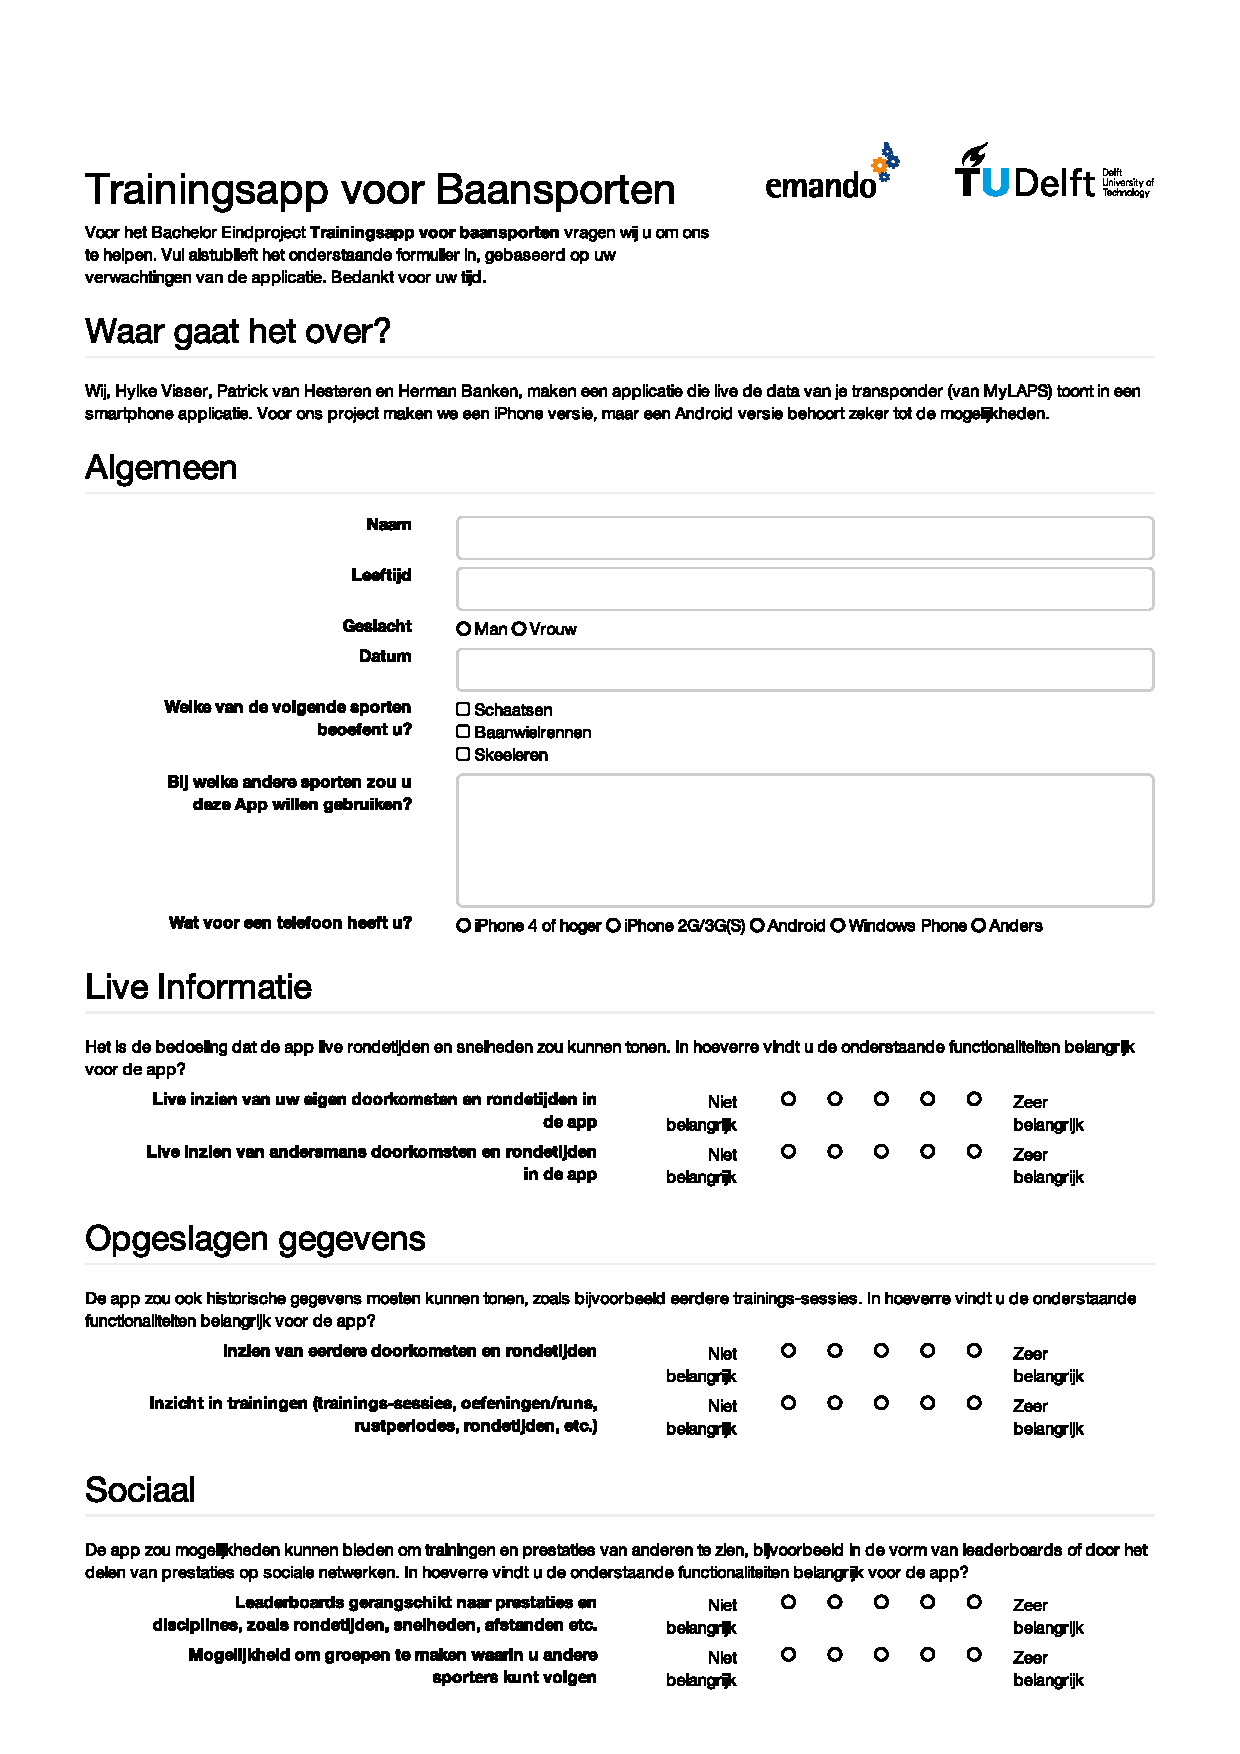
\includegraphics[width=\textwidth]{style/images/Enquete1}
  \end{center}
  \label{fig:enquete1}
\end{figure}

\begin{figure}[ht]
  \begin{center}
    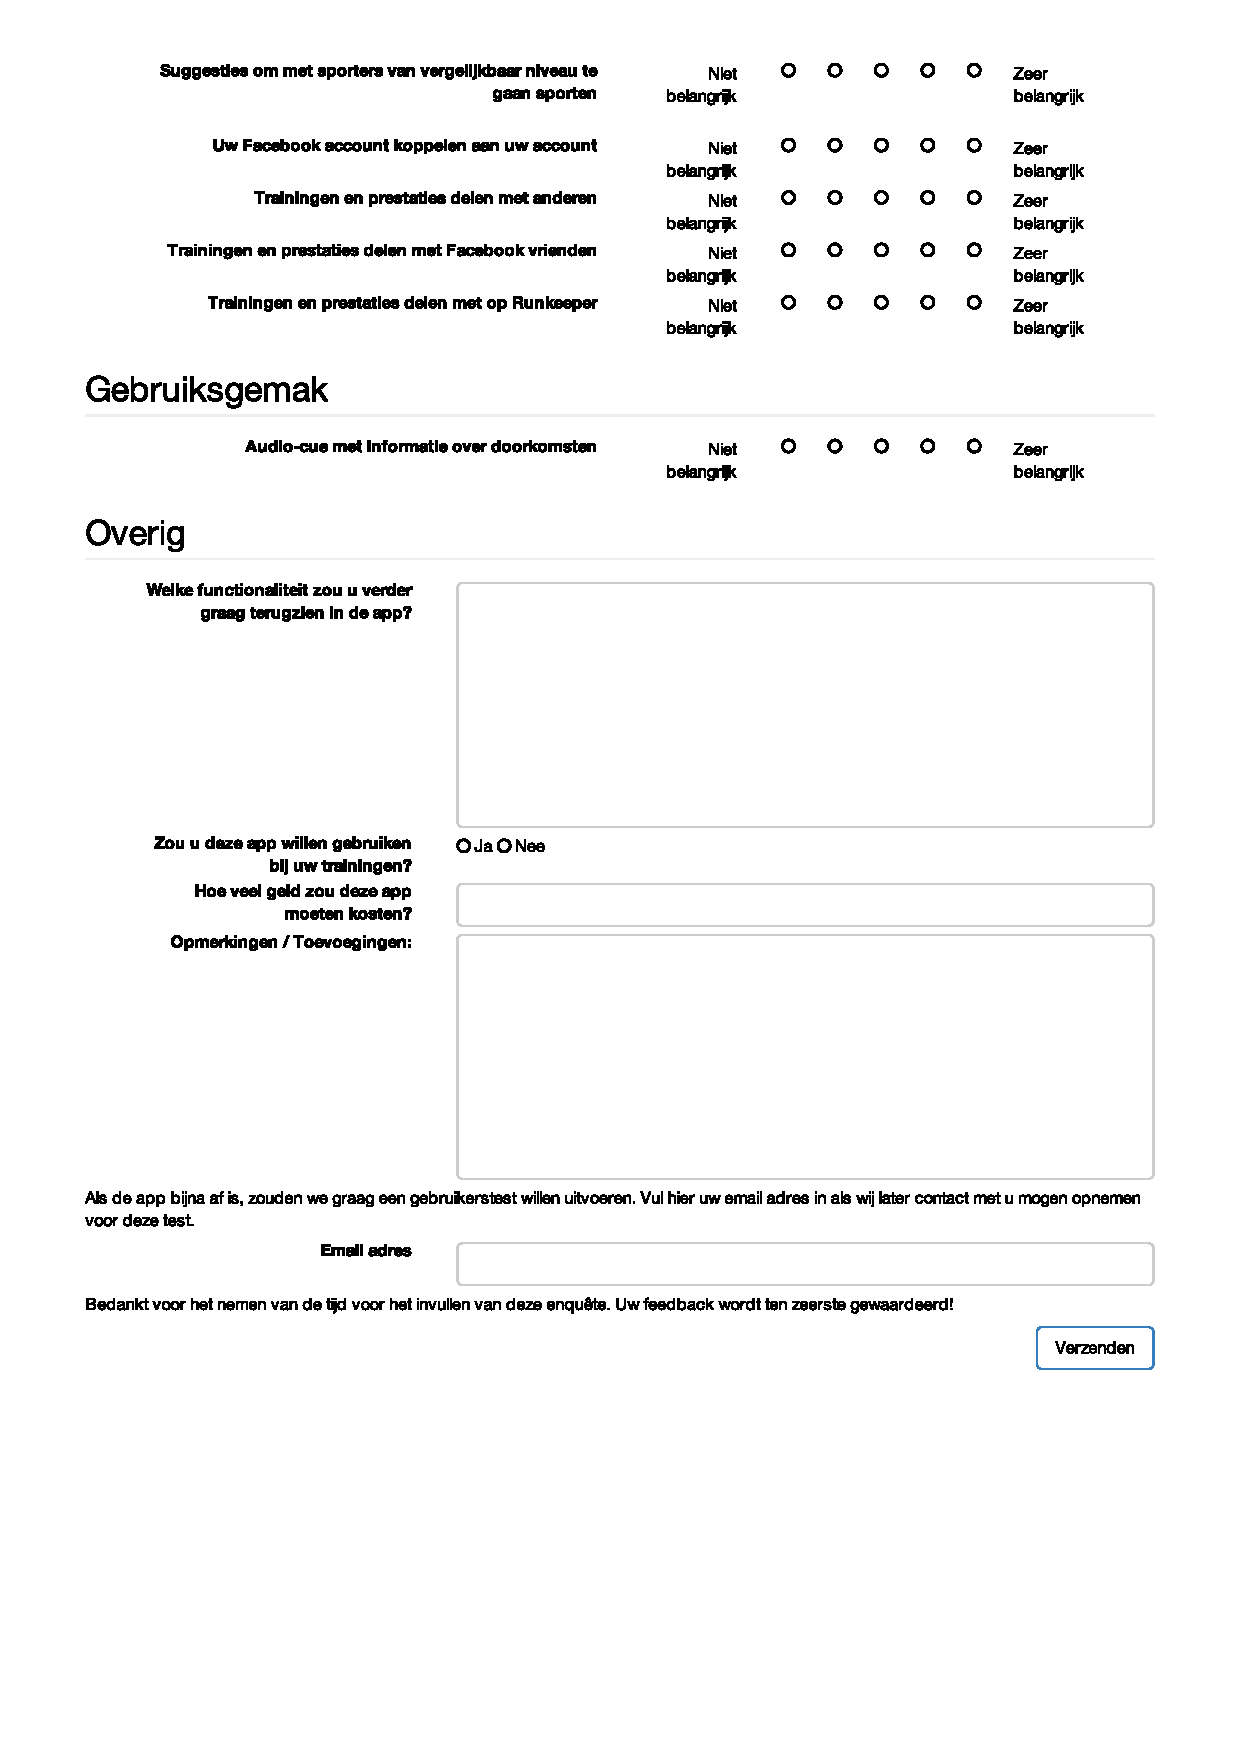
\includegraphics[width=\textwidth]{style/images/Enquete2}
  \end{center}
  \label{fig:enquete2}
\end{figure}

\section{Gebruikerstest}
Op het moment van het plaatsvinden van de gebruikerstest ligt er zomerijs in Thialf. Op ........ zal daarom een gebruikerstest plaats vinden tijdens een reguliere training. We zullen hiervoor de geïnteresseerden die tijdens het invullen van de enquête aangegeven hebben dat ze hieraan graag deelnemen ook uitnodigen.

Tijdens deze reguliere training zullen we hen en andere schaatsers vragen om de applicatie te gebruiken om een test-telefoon. Deze telefoon bevat de applicatie, welke reeds ingesteld is zodat de gebruikers direct aan de slag kunnen met de applicatie. 

\bigskip

Voorafgaand aan de test zullen de testers kort gebrieft worden over de bedoeling van de test. Hierna zal hen gevraagd worden of ze een korte enquête in willen vullen over hun verwachtingen van de applicatie. Ook zal hen worden gevraagd welke aspecten van de applicatie zij belangrijker vinden.

Vervolgens zal de testers gevraagd worden om een serie met (nog te specificeren) acties te verrichten binnen de applicatie. Dit wordt gedaan in de vorm van een Contextual Inquiry~\cite{holtzblatt1993contextual}. Dit houdt in dat de gebruikers tijdens dit proces gevraagd zullen worden om te vertellen wat ze aan het doen zijn en waarom. Het proces zal gefilmd worden voor latere analyse.

Achteraf zullen de gebruikers in een enquête gevraagd worden in hoeverre de acties en functionaliteiten logisch en bruikbaar waren. Ook krijgen ze de mogelijkheid om hierbij opmerkingen te vermelden. Deze enquête zal ook vragen stellen die met behulp van een Likert~Scale~\cite{likert1932technique} beantwoord moeten worden.